\documentclass{beamer}
\usepackage{amsmath}
\usepackage{mathtools}
\usepackage[outline]{contour}

\mode<presentation>
{
  \useoutertheme{default}
}

\beamertemplatenavigationsymbolsempty
\setbeamertemplate{frametitle}[default][center]
%\setbeamercolor{frametitle}{fg=white}
%\setbeamercolor{background canvas}{bg=black}
%\setbeamercolor{normal text}{fg=white}
%\usepackage[dvipsnames]{xcolor}
\definecolor{cyan}{rgb}{0,1,1}
\definecolor{yellow}{rgb}{1,1,0}
\definecolor{magenta}{rgb}{1,0,1}

\title{Downstream analysis: age structure and combinatorial risk factors}
\author{Chay Paterson}
\institute{University of Manchester}
\date{\today}

\begin{document}

\frame{\titlepage}

\begin{frame}
    \frametitle{Outline}
    \begin{enumerate}
        \item Why cancer epidemiology and age structure is interesting (3 slides)
        \item How to study both genomic alterations and age structure
        simultaneously (4 slides)
        \item What data I actually need (2 slides)
    \end{enumerate}
\end{frame}

\begin{frame}
    \frametitle{Age structure and biallelic loss}

    \begin{columns}
        \begin{column}{0.5\textwidth}
            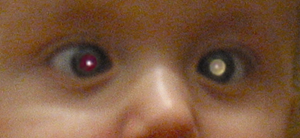
\includegraphics[width=0.90\textwidth]{figures/Rb_whiteeye.PNG}
            \;
            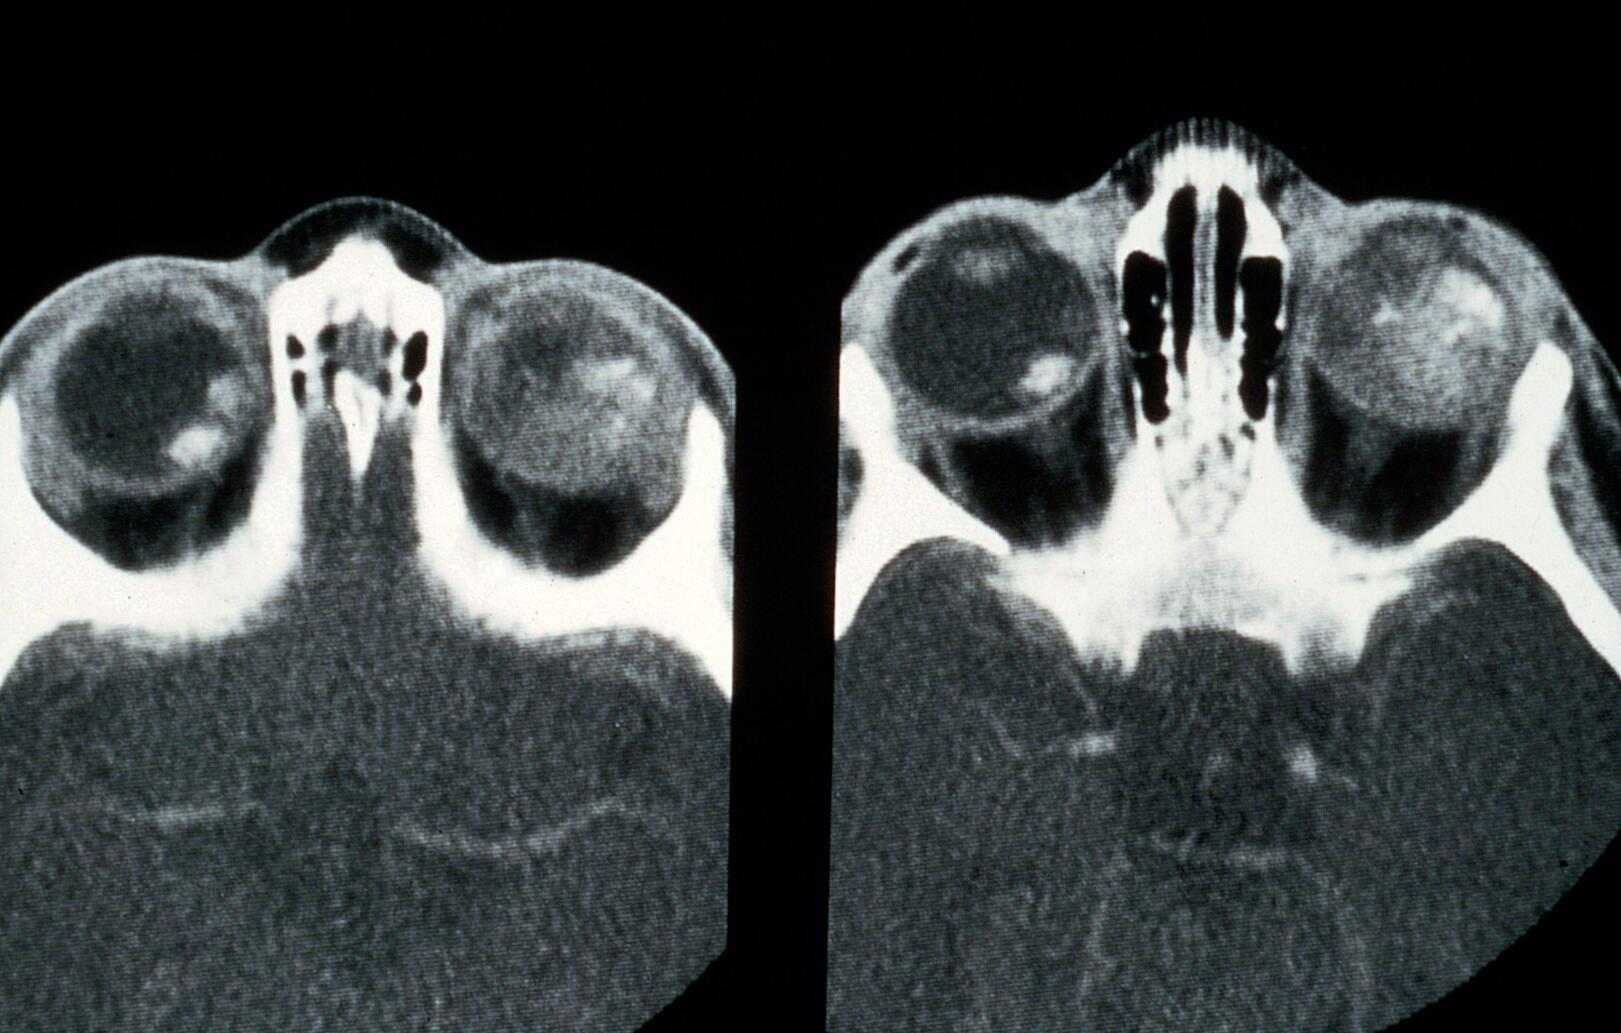
\includegraphics[width=0.90\textwidth]{figures/retinoblastoma.jpg}
            \;
            How many \emph{clonal, rate-limiting} mutations are there?
        \end{column}
        \begin{column}{0.5\textwidth}
            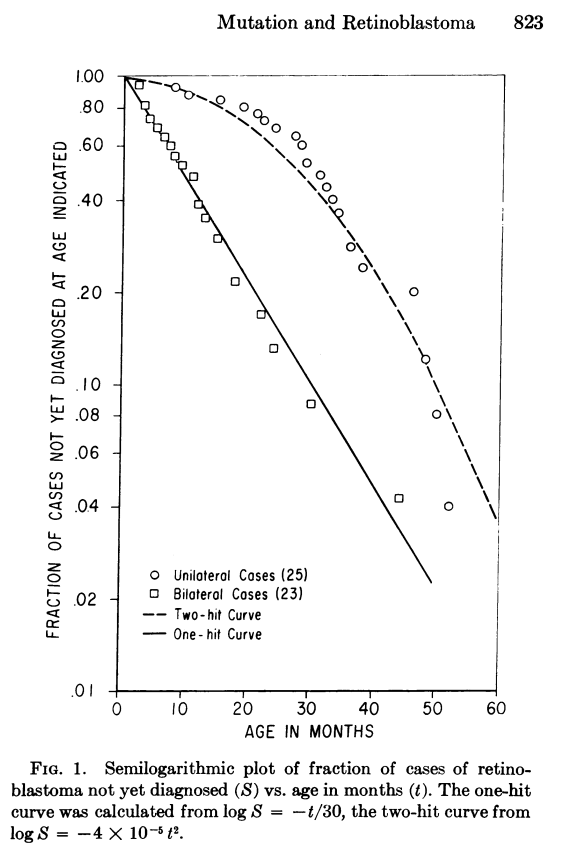
\includegraphics[width=0.90\textwidth]{figures/Screenshot_2022-10-31_11-57-01.png}
        \end{column}
    \end{columns}

\footnotetext[1]{AG. Knudson, PNAS 68.4 (1971): 820-823.}
\footnotetext[2]{F. Michor, Y. Iwasa and MA. Nowak, Nature Reviews Cancer 2004; 4: 197-205 doi:10.1038/nrc1295}
\end{frame}

\begin{frame}
    \frametitle{Classic age structured models}

    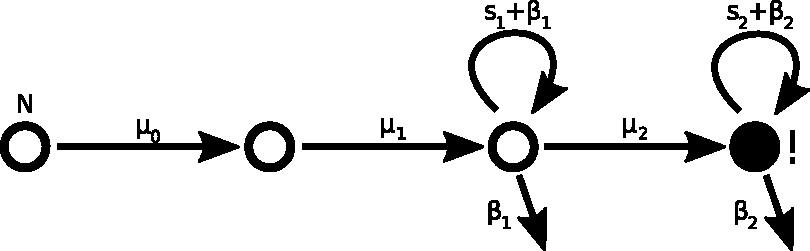
\includegraphics[width=1.00\textwidth]{figures/diagram3}

    \begin{itemize}
        \item The survival curve S(a) determines the incidence curve $I(a)$ 
        \item To fit (or ``train'') the model to longitudinal data, we use a
        model for $S(a)$
        \item Model parameters: mutation rates $\mu_k$, ``fitnesses'' $s_k$, and
        cell turnover/renewal rates $\beta_k$
    \end{itemize}

    \;

    But...
\end{frame}

\begin{frame}
    \frametitle{Limitations of age structured models} 
    Lots of biologically relevant stuff we have learned since doesn't fit into
    these models:

    \begin{enumerate}
        \item can't distinguish between e.g. structural variants and SNVs 
        \item can't distinguish between different orders of events. 
\end{enumerate}

        different combinations of alterations (e.g. loss-of-function indel and
        copy number loss) can result in biallelic loss, but may also
represent different degrees of pathogenicity. IN BRIEF: \emph{genomic} risk factors
\end{frame}

\begin{frame}
    \frametitle{Generalised: Age structured models on graphs}
    \begin{columns}
        \begin{column}{0.5\textwidth}
        \begin{enumerate}
            \item At \textbf{specific loci}, different mechanisms of interest
            (SNVs, LOH, CNA, etc.) can happen in different orders. The different
            combinations of events can be represented with a graph.
            \item We need to evaluate $S(a)$ for a model
            defined on a graph (right)
            \item We have a new algorithm for doing this and getting MLE
            estimates of the parameters
        \end{enumerate}
        \end{column}
        \begin{column}{0.5\textwidth}
        \begin{center}
            \small{example model}
        \end{center}
            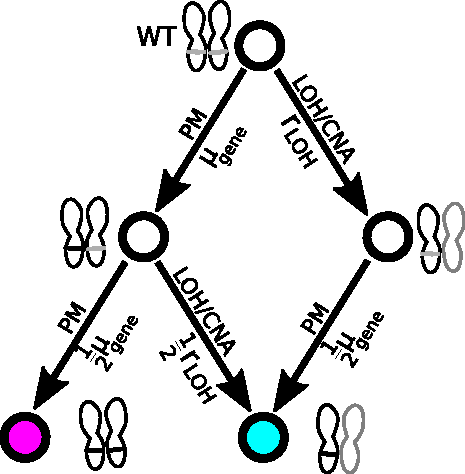
\includegraphics[width=\textwidth]{figures/diagram4}
        \end{column}
    \end{columns}

    \;

    \begin{center}
        This can model the age-incidence of arbitrarily granular subtypes.
        Whatever callers we can run and classify patients, we can get an
        age-incidence curve.
    \end{center}
\end{frame}


\begin{frame}
    \frametitle{Colorectal adenocarcinoma model}
    \begin{columns}
        \begin{column}{0.5\textwidth}
        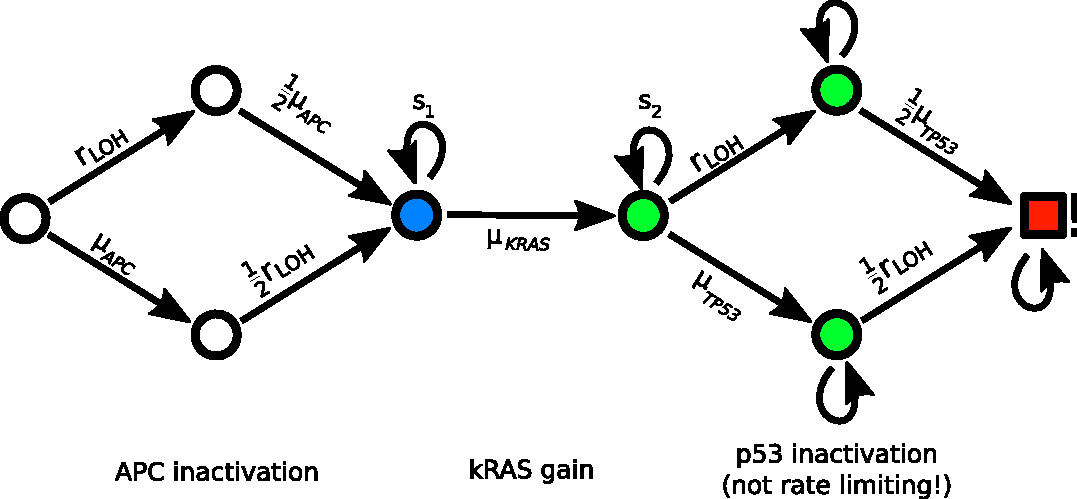
\includegraphics[width=1.0\textwidth]{figures/diagram7}
        \begin{itemize}
            \item Can use A-D type approximation, or stochastic simulations
            %\item Conditional path probabilities $P(X_i)$ encode fitnesses
        \end{itemize}
        but:
        \begin{itemize}
            \item Mean-field breaks down at old ages / large probabilities
            \item Stochastic simulations are \emph{extremely slow}
        \end{itemize}
        \end{column}
        \begin{column}{0.5\textwidth}
        % graph from our PNAS paper
        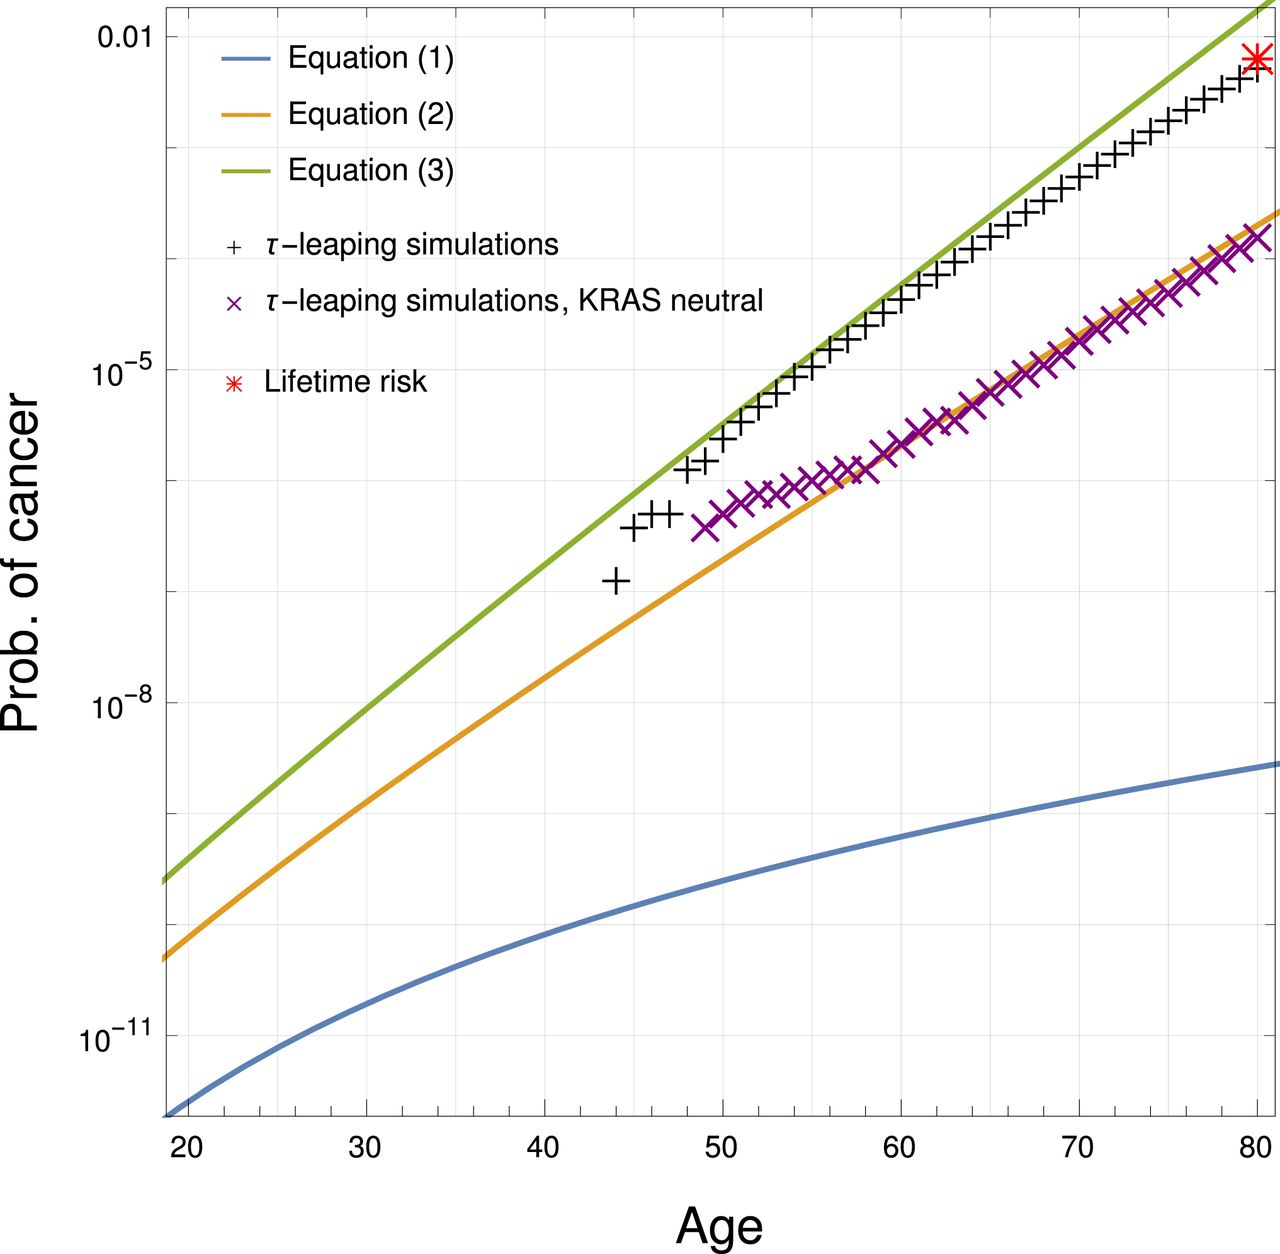
\includegraphics[width=\textwidth]{figures/F2.large.jpg}
        \end{column}
    \end{columns}

\footnotetext[1]{C. Paterson, I. Bozic, H. Clevers, PNAS 2020; 117(34): 20681-20688}
\end{frame}

\begin{frame}
    \frametitle{Kolmogorov forward equations}

    \begin{columns}
        \begin{column}{0.5\textwidth}
    Using the big generating function $\Psi$, find the corresponding wave
    equation:

    \begin{equation}
        \frac{d \Psi}{ dt} = \mathcal{H} \Psi
    \end{equation}

    This can be solved using the method of characteristics, so we can instead
    integrate

    \begin{equation}
        \frac{d \vec{\gamma}}{ dt} = \vec{X}
    \end{equation}
    numerically, using an appropriate time stepper.

        \end{column}
        \begin{column}{0.5\textwidth}
            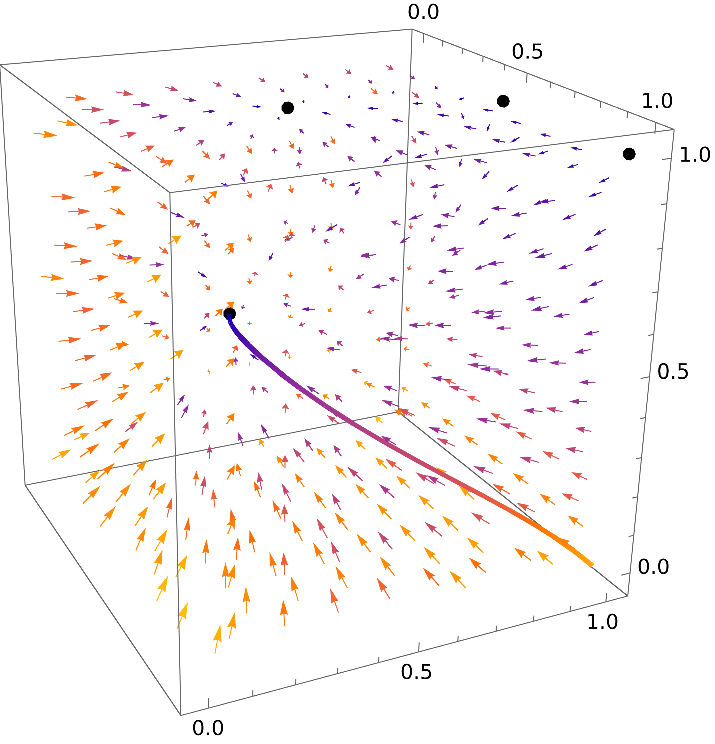
\includegraphics[width=\textwidth]{figures/flowcube1}

            \;

            The vector field $\vec{X}$ and a characteristic $\vec{\gamma}$
        \end{column}
    \end{columns}
\footnotetext[1]{C Paterson, M Gao, J Hellier, G Luebeck, DC Wedge, I
Bo\v{z}i\'{c}, 2025 (pending!)}
\end{frame}

\begin{frame}
    \frametitle{Fast forward method}
    Efficiently computing $S_k(a)$ means we can evaluate likelihood functions
    directly, just sampling them.....

    \framesubtitle{Parameter inference}
    \begin{columns}
        \begin{column}{0.5\textwidth}
        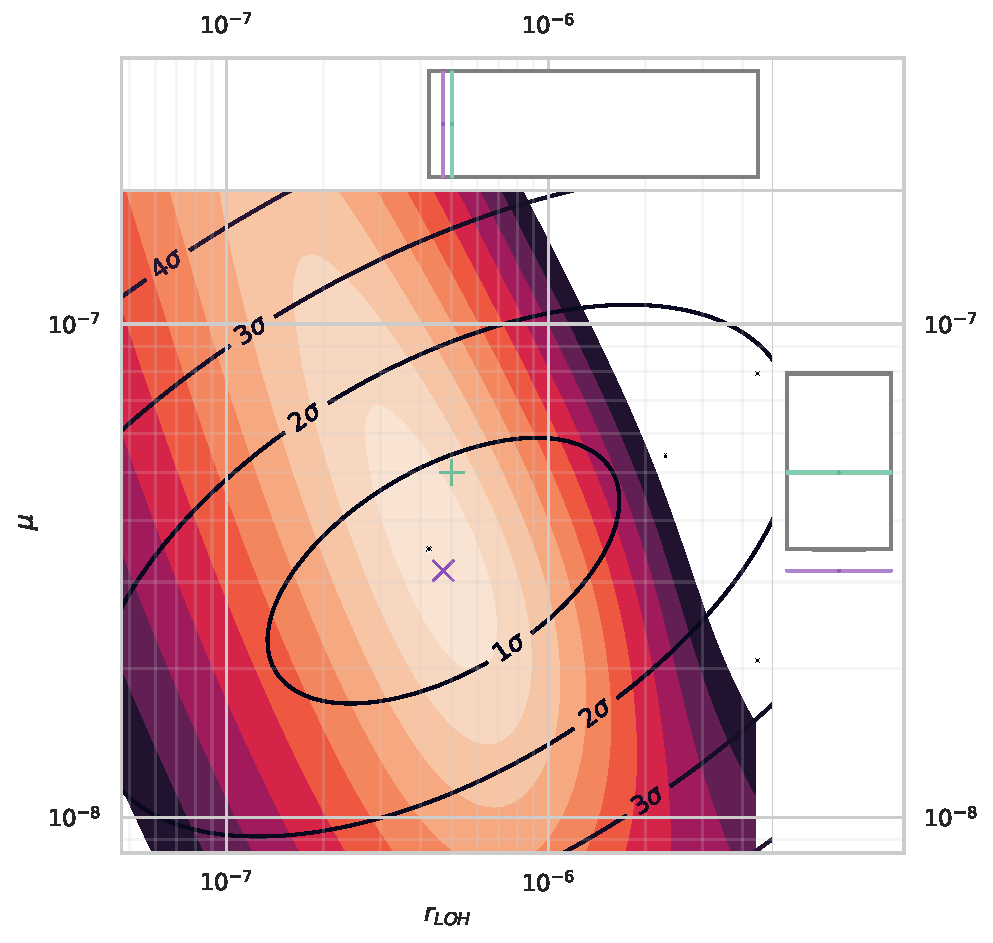
\includegraphics[width=\textwidth]{figures/scatterplot_floating_mutrates_fixed_32}
        \end{column}
        \begin{column}{0.5\textwidth}
        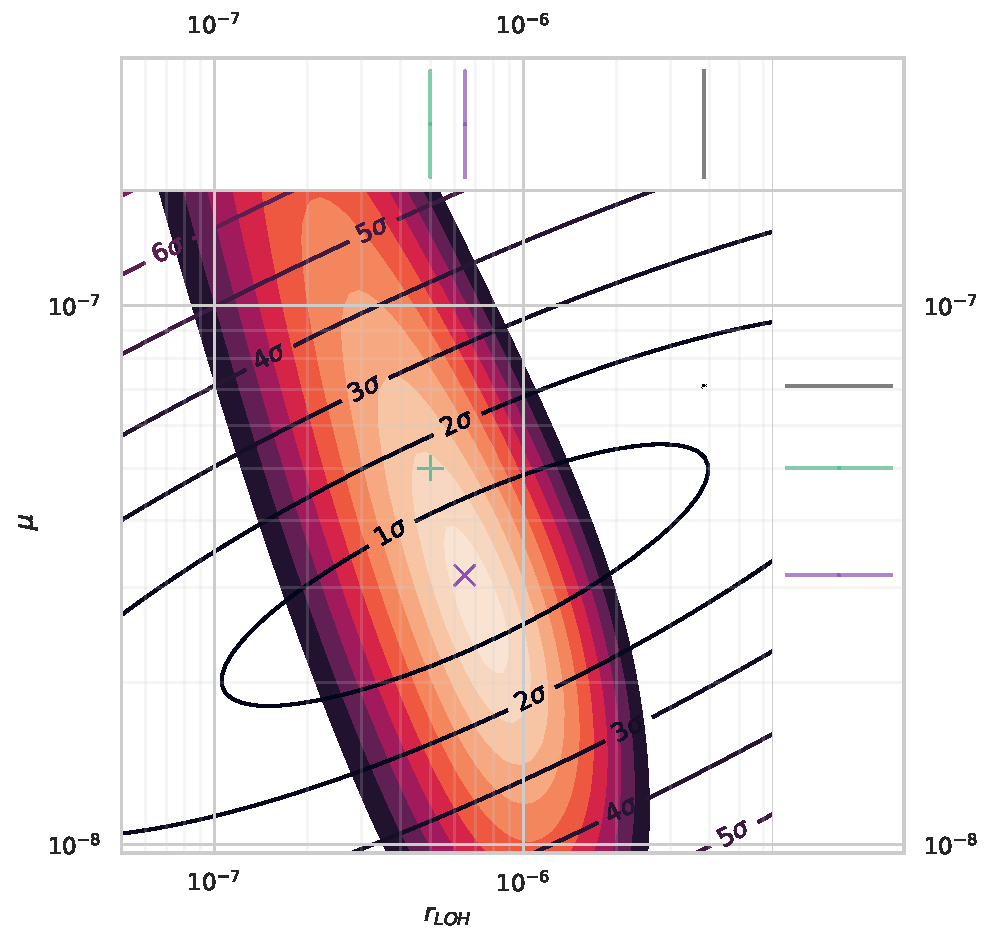
\includegraphics[width=\textwidth]{figures/scatterplot_floating_mutrates_fixed_100}
        \end{column}
    \end{columns}

\footnotetext[1]{C Paterson, M Gao, J Hellier, G Luebeck, DC Wedge, I
Bo\v{z}i\'{c}, 2025 (pending!)}
\end{frame}

\begin{frame}
    \frametitle{What data I actually need}
    Basically, I want to structure on specific alterations. Here's a proposal
    to get us started:

    \begin{itemize}
        \item Focus on p53 (e.g.!) and for each patient with biallelic loss:
        \begin{enumerate}
            \item establish the true WT for each patient as far as possible!
            \item call copy number changes (Battenberg), (non-silent) SNVs (Caveman?), and SVs
            (BRASS?).
            \item consensus?
        \end{enumerate}
        \item Thank you Ginny for the SOP spreadsheet
        \item Battenberg is also partly done (but be careful: back to Marian)
        \item Genomic signatures are also interesting and not locus-specific:
        I'm especially interested in seeing SBS1 called as it's clock-like.
    \end{itemize}

\end{frame}

\begin{frame}
    \frametitle{What data I actually need}
    End result should be (for each locus of interest) a ``spreadsheet'' that looks
    like:

    \begin{center}
    \tiny{
    \begin{tabular}{| l | l | l | l | l | l | l | l |}
    \hline
    Patient ID & Age at diag. & 17p major CN & 17p minor CN & SV (over p53) &
    SNV (on p53) & indels... & \dots \\
    \hline
    B120002 & 68 & 2 & 0 & None & ...TCG$>$TAG... & \dots & \dots \\
    \hline
    B120005 & 54 & 2 & 1 & None & None & such\&such & \dots \\
    \hline
    \dots & \dots & \dots & \dots & \dots & \dots & \dots & \dots \\
    \hline
    \end{tabular}

    }
    \end{center}

    NB: This ``row'' can be continued for any other loci/gene of interest.

    \;
    
    Each column heading (except ID and age) becomes an edge on the graph and
    each combination of events becomes a final node on the graph. (Continuing the
    table corresponds to taking a Kronecker product of multiple graphs)
\end{frame}

\end{document}
